\section{\uppercase{Results}}
\label{sec:results}
\subsection{Data} \label{sec:unitroot}
Tests of SLVECM, SLARIMA and our proposal OVECM were carried out using foreign
four exchange data rates: EURUSD, GBPUSD, USDCHF and USDJPY. This data was
collected from the free database Dukascopy which gives access to the Swiss
Foreign Exchange Marketplace ~\cite{Dukascopy2014}.

The reciprocal of the last two rates (CHFUSD, JPYUSD) were used in order to
obtain the same base currency for all rates.  The tests were done using
1-minute frequency from ask prices which corresponded to 1.440 data points per
day from the 11th to the 15th of August 2014.

\subsection{Unit root tests} \label{sec:unitroot}
Before running the tests, we firstly checked if they were I(1) time series
using the Augmented Dickey Fuller (ADF) test.

\begin{table}[h!]
\caption{Unit roots tests}
\label{tab:adf}
\begin{center}
\begin{tabular}{|l|c|c|c|c|c|}
\hline
& \textbf{Statistic} & \textbf{Critical value} & \textbf{Result}\\
\hline
EURUSD          & -0.64 & -1.94 & True       \\
$\Delta$EURUSD & -70.45   & -1.94 & False       \\
GBPUSD          & -0.63   & -1.94 & True          \\
$\Delta$GBPUSD & -54.53   & -1.94 & False       \\
CHFUSD          & -0.88   & -1.94 & True         \\
$\Delta$CHFUSD & -98.98   & -1.94 & False       \\
JPYUSD          & -0.65 & -1.94 & True        \\
$\Delta$JPYUSD & -85.78 & -1.94 & False     \\ 
\hline
\end{tabular}
\end{center}
\end{table}


Table~\ref{tab:adf} shows that all currency rates cannot reject the unit root
test but they rejected it with their first differences. This means that all of
them are I(1) time series and we are allowed to use VECM and therefore OVECM.


\subsection{Parameter selection} \label{sec:paramselection}

In order to set OVECM parameters: windows size $L$ and lag order $p$,
we propose to use several window sizes: $L = 100, 400, 700, 1000$. For every window size $L$ we chose lag order with minimum AIC.

ARIMA parameters were also obtained using AIC.
Parameters optimization is presented in table~\ref{tab:params}:

\begin{table}[ht]
\caption{Parameters optimization. VECM order and ARIMA parameters were selected
using AIC.}
\label{tab:params}
\begin{center}
\begin{tabular}{|c|c|c|}
\hline
Windows size $L$ & VECM & ARIMA\\
 $L$ & order $(p)$ & order $(p,d,q)$ \\
\hline
100 & 2 & p=2,d=1,q=1\\
400 & 5 & p=1,d=1,q=1\\
700 & 3 &p=2,d=1,q=1\\
1000 &3 & p=2,d=1,q=1\\
\hline
\end{tabular}
\end{center}
\end{table}

In OVECM we also define a mean\_error variable, which was defined based on the
in-sample MAPEs. Figure \ref{fig:mapes} shows how MAPE moves and how mean\_error
variable help us to decide whether new cointegration vectors are needed.

\begin{figure}[!h]
  \centering
   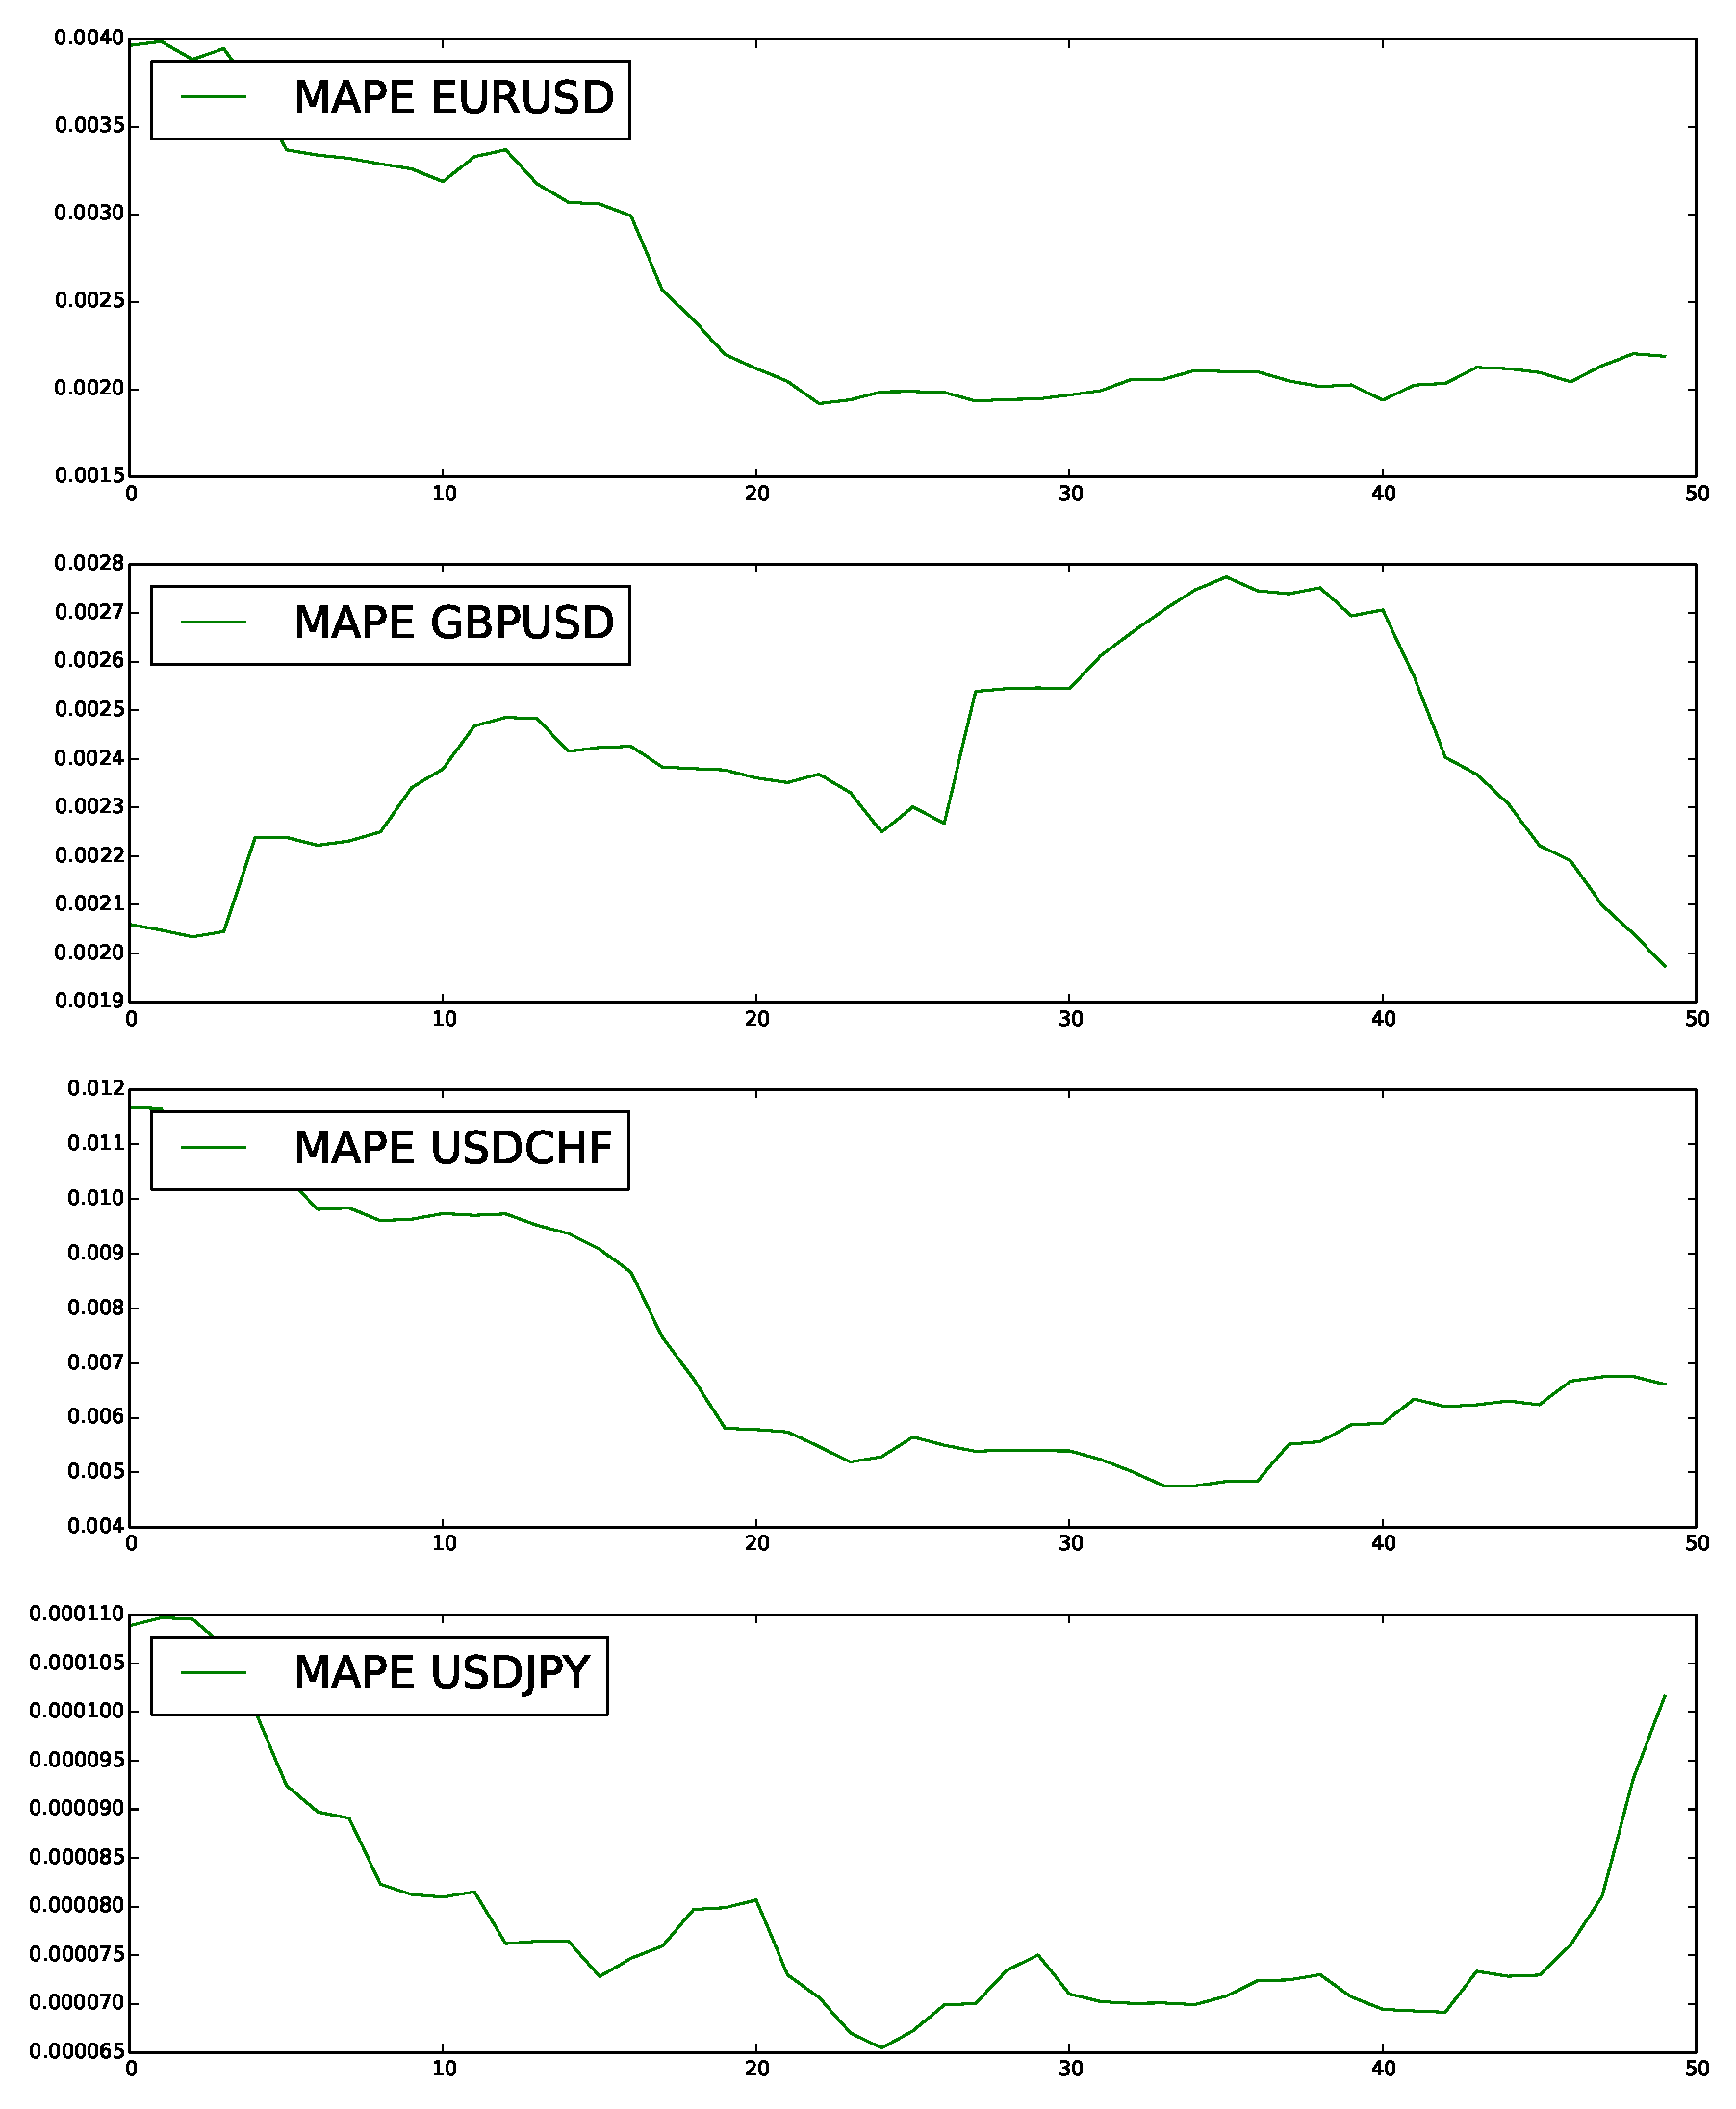
\includegraphics[width = 7.5cm]{img/mapes} 
  \caption{In-sample MAPEs example for 50 minutes. The average of them is
  considered to obtain new cointegration vectors.}
  \label{fig:mapes}
 \end{figure}



\subsection{Execution times} \label{sec:exectimes}
We ran OVECM and SLVECM 400 iterations. SLARIMA execution time is excluded
because its is not comparable with OVECM and SLVECM. SLARIMA was created based
on statsmodels library routine ARIMA.

The execution times are shown in the table~\ref{tab:extimes}.

\begin{table}[h!]
\caption{Execution times}
\label{tab:extimes}
\begin{center}
\begin{tabular}{|l|c|c|c|c|c|}
\hline
& $L$ & order & e  & Time[s] \\
\hline
OVECM & 100 &p=2  & 0      & 2.492\\
OVECM & 100 &p=2  & 0.0026  & 1.606\\
SLVECM & 100 &p=2& -- & 2.100\\
\hline
OVECM & 400 & p=5  & 0      & 3.513\\
OVECM & 400 &p=5  & 0.0041  & 2.569\\
SLVECM & 400 & p=5 & -- & 3.222\\
\hline
OVECM & 700 &p=3  & 0      & 3.296\\
OVECM & 700 &p=3  & 0.0032  & 2.856\\
SLVECM & 700 &p=3 & -- & 3.581\\
\hline
OVECM & 1000 & p=3 & 0      & 4.387\\
OVECM & 1000 & p=3  & 0.0022  & 2.408\\
SLVECM & 1000 & p=3  & -- & 3.609\\
\hline
\end{tabular}
\end{center}
\end{table}

It is clear that execution time depends directly on $L$ and $p$ since they
determine the size of matrix $\mathbf{A}$ and therefore affect the OLS function
execution time.
It is worthy of note that execution time also depends on mean\_error because it
determines how many times OVECM will recalculate cointegration vectors which is
an expensive routine.

Figure~\ref{fig:mapes} shows an example of the in-sample MAPE for 50 iterations.
When the average of the in-sample MAPEs is above mean\_error new cointegration
vectors are obtained. In consequence, OVECM performance increases when
mean\_error increases. However, this could affect accuracy, but
table~\ref{tab:stats} shows that using an appropriate mean\_error doesn't affect
accuracy considerable. 

\subsection{Performance accuracy} \label{sec:performacc}

Table~\ref{tab:stats} shows in-sample and out-of-sample performance measures:
MAPE, MAE and RMSE for OVECM, SLVECM and SLARIMA. Test were done using the
parameters defined in table \ref{tab:params}.  We can see that OVECM has very
similar performance than SLVECM and this support the theory that cointegration
vectors vary little in time. Moreover, OVECM also out performed SLARIMA based on
these three performance measures. 


\begin{table*}[ht!]
\caption{Model measures}
\label{tab:stats}
\begin{center}
\begin{tabular}{|l|l|c|c|c|c|c|c|c|c|}
\hline
\multicolumn{4}{|c|}{Model} & \multicolumn{3}{|c|}{In-sample} &
\multicolumn{3}{|c|}{Out-of-sample} \\ 
\hline
\hline
Method & $L$ & Parameters & e & 
MAPE & MAE& RMSE& 
MAPE & MAE& RMSE \\
\hline
 OVECM  &   100  &  P=2& 0.0026  &  0.00263&  0.00085&  0.00114&  0.00309&  0.00094&  0.00131\\
 OVECM  &   400  &  P=5& 0.0041  &  0.00378&  0.00095&  0.00127&  0.00419&  0.00103&  0.00143\\
 OVECM  &   700  &  P=3& 0.0032  &  0.00323&  0.00099&  0.00130&  0.00322&  0.00097&  0.00132\\
 OVECM  &   1000 &  P=3& 0.0022  &  
 \textbf{0.00175}&  \textbf{0.00062}&  \textbf{0.00087} &  
 \textbf{0.00172}&  \textbf{0.00061}&  \textbf{0.00090}\\
\hline
 SLVECM  &   100 &  P=2& -  &  0.00262&  0.00085&  0.00113&  0.00310&  0.00095&  0.00132\\
 SLVECM  &   400 &  P=5& -  &  0.00375&  0.00095&  0.00126&  0.00419&  0.00103&  0.00143\\
 SLVECM  &   700 &  P=3& -  &  0.00324&  0.00099&  0.00130&  0.00322&  0.00098&  0.00132\\
 SLVECM  &   1000 &  P=3& -  &  
 \textbf{0.00174}&  \textbf{0.00061}&  \textbf{0.00087}&  
 \textbf{0.00172}&  \textbf{0.00061}&  \textbf{0.00090}\\
\hline
SLARIMA & 100  &p=2, d=1, q=1 & - & 0.00285  &  0.00110  &  0.00308  &  0.00312  &0.00098  &  0.00144 \\
SLARIMA & 400  &p=1, d=1, q=1 & - & 0.00377  &  0.00101  &  0.00128  &  0.00418 & 0.00106 & 0.00145 \\
SLARIMA & 700  &p=2, d=1, q=1 & - & 0.00329  &  0.00102  &  0.00136  &  0.00324  & 0.00097  &  0.00133 \\
SLARIMA & 1000 &p=2, d=1, q=1 & - & \textbf{0.00281}  & \textbf{0.00074}  &  \textbf{0.00105}  &  \textbf{0.00177} & \textbf{0.00063}  &  \textbf{0.00092} \\
\hline
\end{tabular}
\end{center}
\end{table*}

We can also notice that in-sample performance in OVECM and SLVECM is related
with the out-of-sample performance.  This differs with SLARIMA which models with
good in-sample performance are not necessarily good out-of-sample models.
Moreover OVECM outperformed SLARIMA using the same window size.

Figure ~\ref{fig:accuracy} shows the out-of-sample forecasts made by our
proposal OVECM with the best parameters found based on table~\ref{tab:stats}
which follows the time series very well.  

\begin{figure}[h]
  \vspace{-0.2cm}
  \centering
   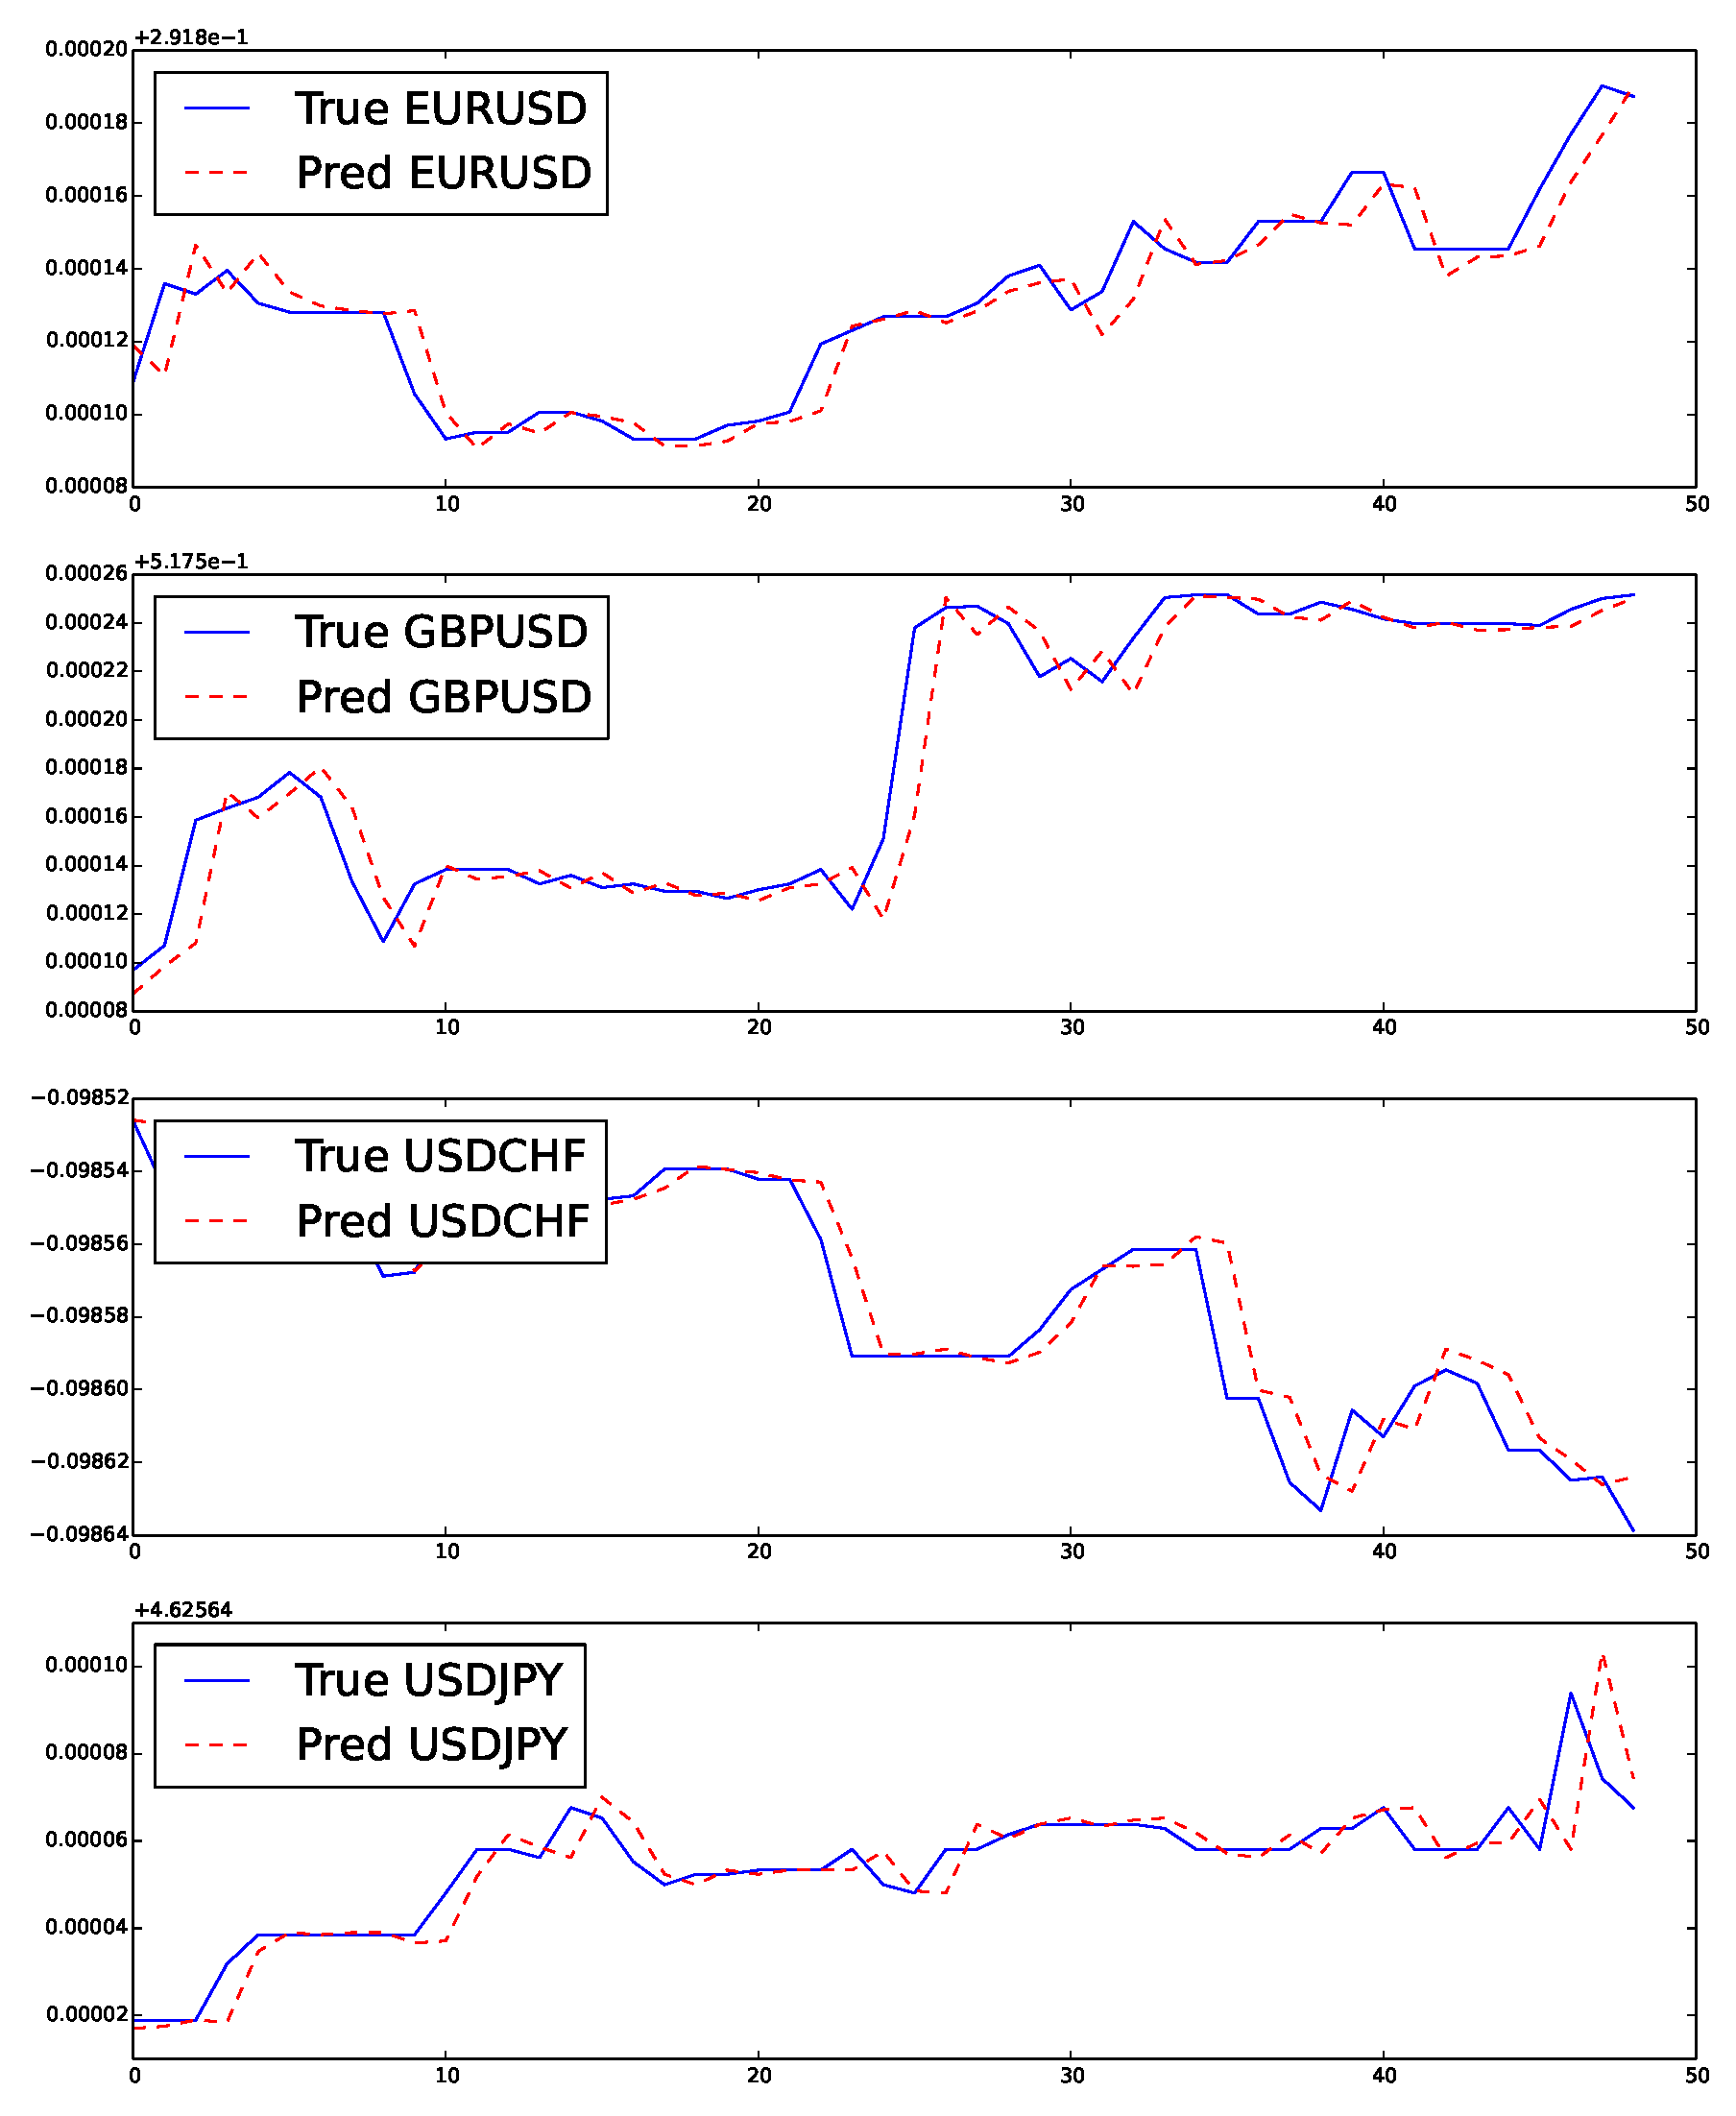
\includegraphics[width = 7.5cm]{img/accuracy} 
  \caption{OVECM forecasting accuracy example for 50 minutes using $L = 1000$ and $p =3$}
  \label{fig:accuracy}
 \end{figure}


